\documentclass{article}
\usepackage[utf8]{inputenc}
\usepackage[spanish]{babel}
\usepackage{graphicx}
\usepackage{anysize}
\usepackage{fancyhdr} 
\usepackage[export]{adjustbox}
\usepackage{titlesec}
\usepackage{enumitem}
\usepackage{listings}
\usepackage{xcolor}

% \usepackage{hyperref}
% \usepackage{float}
% \usepackage{tabu}

% Izquierda, derecha, arriba, abajo
\marginsize{2cm}{2cm}{1.2cm}{1.5cm} 
\renewcommand{\familydefault}{\sfdefault}
\decimalpoint%

\graphicspath{{assets/}}

\setlength{\parindent}{0in}
\titleformat*{\section}{\large\bfseries}

% Para insert código
\definecolor{codegreen}{rgb}{0,0.6,0}
\definecolor{codegray}{rgb}{0.5,0.5,0.5}
\definecolor{codepurple}{rgb}{0.58,0,0.82}
\definecolor{backcolour}{rgb}{1,1,1}

\usepackage{textcomp}
\lstset{upquote=true}
\lstdefinestyle{mystyle}{
    backgroundcolor=\color{backcolour},   
    commentstyle=\color{codegreen},
    keywordstyle=\color{magenta},
    numberstyle=\tiny\color{codegray},
    stringstyle=\color{codepurple},
    basicstyle=\ttfamily\footnotesize,
    breakatwhitespace=false,         
    breaklines=true,                 
    captionpos=b,                    
    keepspaces=true,                 
    % numbers=left,                    
    % numbersep=5pt,                  
    showspaces=false,                
    showstringspaces=false,
    showtabs=false,                  
    tabsize=2
}

\lstset{style=mystyle}

\newcommand{\materia}{BDA}
\newcommand{\clave}{2929}
\newcommand{\profesor}{Ing. Rodriguez Campos \textsc{Jorge Alberto}}
\newcommand{\grupo}{1}
\newcommand{\semestre}{2021-1}

\newcommand{\alumno}{Francisco Pablo \textsc{Rodrigo}}

\newcommand{\actividad}{Tema 02 \\ Ejercicio práctico 04}
\newcommand{\titulo}{Administración de parámetros}

\newcommand{\fechaEntrega}{2 de noviembre de 2020}

%%%%%%%%%%%%%%%%%%%% ENCABEZADO %%%%%%%%%%%%%%%%%%%%%%%%%%%%
\pagestyle{fancy}
\fancyhf{}
\renewcommand{\headrulewidth}{0pt}
\fancyhead[R]{% Left header
    \begin{tabular}{l}
        \materia \\ 
        \actividad%
    \end{tabular}
    \,% Space
    \rule[-1.75\baselineskip]{0pt}{0pt}
    % Strut to ensure a 1/4 \baselineskip between image and header rule
    
\includegraphics[height=3\baselineskip,valign=c]{unam}
}
\setlength{\headsep}{0.3in}


\begin{document}
%%%%%%%%%%%%%%%%%%% DATOS PORTADA %%%%%%%%%%%%%%%%%%%%%%%%
\thispagestyle{empty}
\begin{minipage}[t][5cm][t]{0.2\linewidth}
    
\includegraphics[width=2.5cm]{unam.jpg}
    \vspace{10cm}

    
\includegraphics[width=2.5cm]{fiblack}
\end{minipage}
\begin{minipage}[t]{0.7\linewidth}
    \vspace{-2.5cm}
    \LARGE{\textbf{Universidad Nacional Autónoma de México}}\\
    \Large{\textbf{Facultad de Ingeniería}} \\

    \large{\semestre}\\[2cm]

    \large{\textbf{\materia (\clave)}}\\
    \large{\textbf{Gpo: 1}}\\[5mm]
    \large{\textbf{Profesor:} \profesor}\\ [1.5cm]
    \begin{center}
        \LARGE{\textbf{\actividad}}\\
        \LARGE{\textbf{\titulo}}\\
    \end{center}

    \vspace{3.3cm}

    \large{\textbf{Alumno:} \alumno} \\[1.5cm]

    \begin{flushright}
        \fechaEntrega%
    \end{flushright}
\end{minipage}

\newpage
%%%%%%%%%%%%%%%%%%% CONTENIDO %%%%%%%%%%%%%%%%%%%%%%%%

\section*{Objetivos}
Comprender y poner en práctica os conceptos asociados con la configuración de 
los parámetros de una base de datos, en particular, los 3 niveles de
aplicación: nivel sesión, nivel instancia y nivel SPFILE, así como las 
diferentes opciones que existen para obtener y reconstruir tanto PFILEs como 
SPFILEs.

\section*{C1. Código del script \texttt{s-00-crea-directorios.sh}}
\lstinputlisting[language=Bash]
    {tema02-ej-prac-04-codigo/s-00-crea-directorios.sh}

\section*{C2. Código del script \texttt{e-01-spparameter-alert-log.txt}}
\lstinputlisting[language=Bash,firstline=57,lastline=70]
    {tema02-ej-prac-04-codigo/e-01-spparameter-alert-log.txt}
\section*{C3. Respuestas de las preguntas referentes al contenido de 
los archivos PFILE.}
\begin{enumerate}
    \item Observar que los parámetros mostrados en el archivo 
    \texttt{e-02-spparameter-pfile.txt} tienen 2 formatos: algunos inician con
    \texttt{<oracle\_sid>.\_\_} y otro grupo inicia con \texttt{*.} ¿Qué 
    diferencia existe entre estos 2 grupos?\\
    
    Como el spfile se creo a partir de una instancia levantada con un pfile,
    podemos observar que los parámetro que inician con \texttt{*.} representan
    a aquellos que ya estaban configurados en el pfile. Por otra parte, como
    ya se dijo, este spifle se creo a partir de una instancia que tenía ciertos
    parámetros por ello son los vemos con notación \texttt{<oracle\_sid>.\_\_}
    \item Comparar los 2 archivos \texttt{e-01-spparameter-alert-log.txt} y 
    \texttt{e-02-spparameter-pfile.txt} así como el contenido de la tabla
    \texttt{t01\_spparameters}. Confirmar que en los 3 casos, existen los mismos 
    parámetros con los mismos valores. De encontrar diferencias mencionarlas.\\

    La única diferencia visible es que en la tabla los datos de la memoria estan
    almacenados en kilobyes, fuera de eso, en todas las fuentes de consulta 
    son idénticas.
\end{enumerate}
\newpage
\section*{C4. Contenido parcial del archivo \texttt{e-03-spparameter-pfile.txt}}
\lstinputlisting[language=Bash,firstline=13]
    {tema02-ej-prac-04-codigo/e-03-spparameter-pfile.txt}
\section*{C5. Salida del validador de cambio de parámetros.}
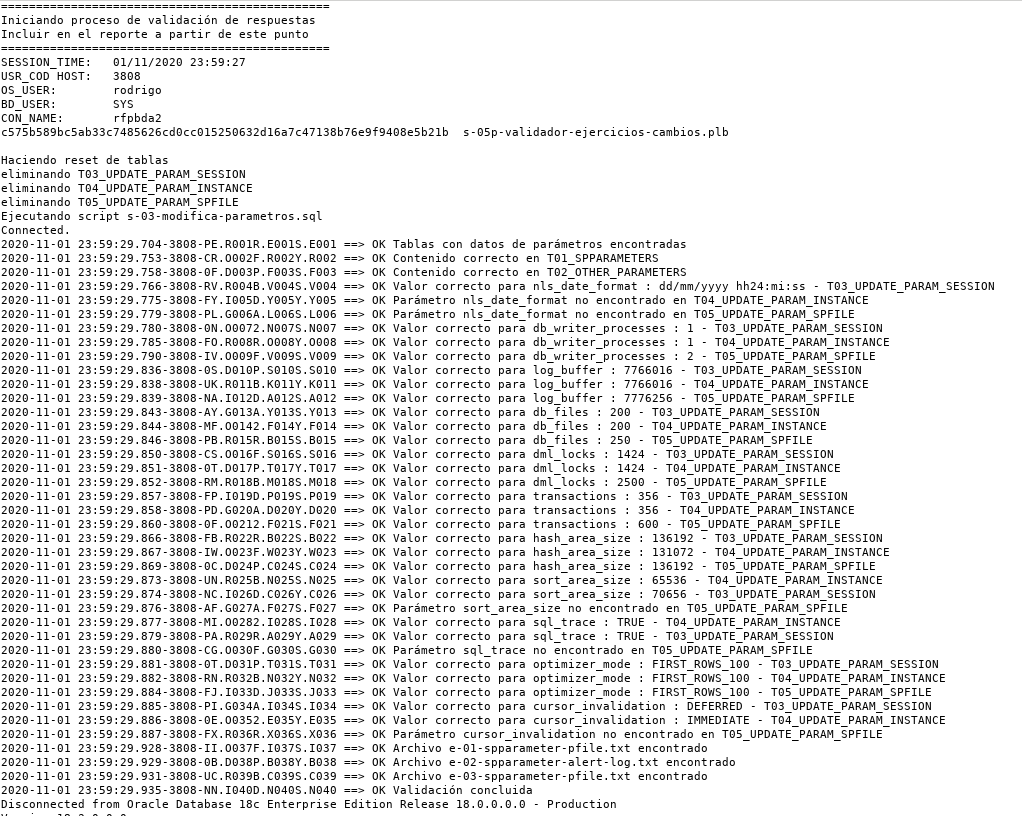
\includegraphics[width=\linewidth]{tema02-ej-prac-04-part01-validador.png}
\section*{C6. Salida del validador de restauración de parámetros.}
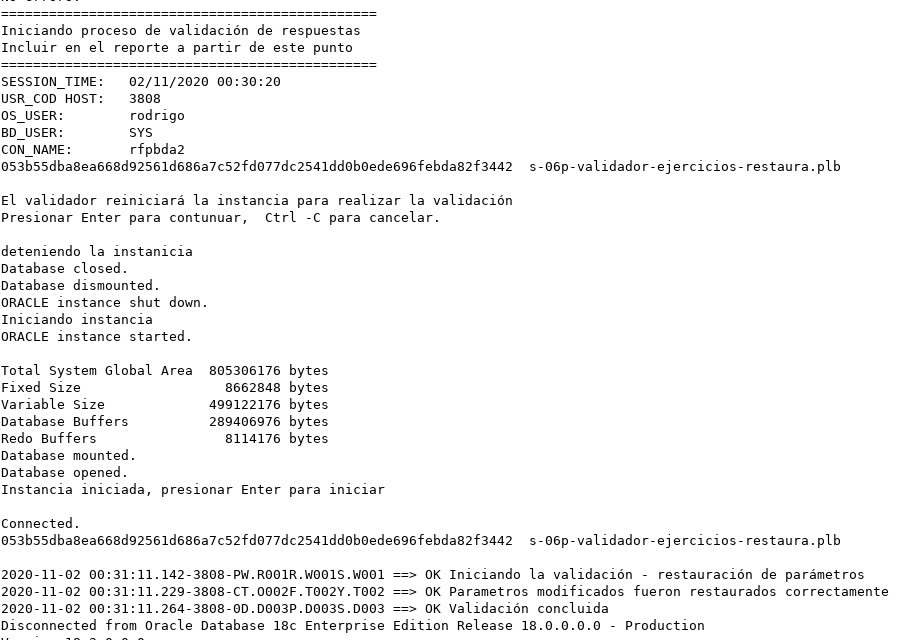
\includegraphics[width=\linewidth]{tema02-ej-prac-04-part02-validador.png}
\section*{Comentarios y conclusiones}

En esta práctica aprendimos a estar preparados para perder y recuperar el
archivo de parámetros en caso de que este se llegué a corromper. 
Aprendimos varias formas de recuperarlo, por ejemplo, si la instancia esta 
levantada podemos realizar el respaldo de los parámetros que se encuentran en
memoria. Otra forma útil de recuperar la configuración de los parámetros cuando
todas las opciones parecen haberse terminado es buscar los parámetros en el 
archivo de \textit{alert log}.

\renewcommand\refname{Bibliografía y referencias}
\begin{thebibliography}{99}
    \bibitem{burleson} Burleson Consulting. \textit{Oracle tips } en 
    \texttt{http://www.dba-oracle.com/oracle\_news/}
    \bibitem{halo}  Halo Linux Services. \textit{Creating a Server Parameter 
    File SPFILE} en 
    \texttt{https://www.halolinux.us/oracle-dba/
    creating-a-server-parameter-file-spfile.html}
    \bibitem{oraclebase} ORACLE-BASE. \textit{Persistent Initialization 
    Parameters} en 
    \texttt{
        https://oracle-base.com/articles/9i/\\
        persistent-initialization-parameters
    }
\end{thebibliography}

\end{document}
